\documentclass{article} % For LaTeX2e
\usepackage{style-file,times}
\usepackage{hyperref}
\usepackage{url}
\usepackage{graphicx}
\usepackage[numbib,notlof,notlot,nottoc]{tocbibind}
\usepackage{enumitem}

\title{Project Milestone: Generating Playlist Names using Tracklist Information}

\author{
    Team: Sofia Samaniego de la Fuente (SUID: sofiasf) \\
    \texttt{\footnotesize sofiasf@stanford.edu}\\ 
    Mentor: Richard Socher
}

\newcommand{\fix}{\marginpar{FIX}}
\newcommand{\new}{\marginpar{NEW}}

\nipsfinalcopy % Uncomment for camera-ready version

\begin{document}
\maketitle

%\begin{abstract}
%\end{abstract}

\section{Problem Description}
\label{description}
The goal is to implement a model that generates a name for a playlist given information about its tracklist. 
In particular, we will attempt to construct a network that builds an internal representation of the names of the tracks included in the playlist and then uses natural language generation techniques to come up with a title that could be close to one a human might devise. 

\section{Data}
\label{data}
Spotify recently released the \emph{Million Playlist Dataset}, official website hosted at \href{https://recsys-challenge.spotify.com}{https://recsys-challenge.spotify.com}, as part of its 2018 RecSys Challenge.
It comprises a set of $1,000,000$ playlist that have been created by Spotify users along with a variety of features, including playlist name, description, timestamp when the playlist was last updated, and an array of information about each track in the playlist (track name, artist, album name, duration, position in the playlist).
Additionally, Spotify provides a \textsf{python} script that computes the following statistics for the dataset:

\begin{table}[h!]
\caption{Statistics for the \emph{Million Playlist Dataset}}
\centering
 \begin{tabular}{|lr|} 
 \hline
 	Number of playlists & 1,000,000 \\
	Number of tracks & 66,346,428 \\
	Number of unique tracks & 2,262,292 \\
	Number of unique albums & 734,684 \\
	Number of unique artists & 295,860 \\
	Number of unique titles & 92,944 \\
	Number of playlists with descriptions & 18,760 \\
	Number of unique normalized titles & 17,381 \\
	Avg playlist length & 66.346428 \\     
 \hline
 \end{tabular}
\end{table}

\begin{table}[h!]
\caption{Top playlist names, artists, and songs (with counts)}
\centering
  \begin{tabular}{|c|c|c|} 
  	\hline 
  	Playlist Title & Track & Artist \\
  	\hline
  	Country  & HUMBLE. by Kendrick Lamar  & Drake  \\ 
  	Chill  & One Dance by Drake  & Kanye West  \\
  	Rap  & Broccoli (feat. Lil Yachty) by DRAM  & Kendrick Lamar  \\
  	Workout  & Closer by The Chainsmokers  & Rihanna  \\
  	Oldies  & Congratulations by Post Malone  & The Weeknd  \\
  	Christmas  & Caroline by Aminé  & Eminem  \\
  	Rock  & iSpy (feat. Lil Yachty) by KYLE  & Ed Sheeran  \\
  	Party  & Bad and Boujee (feat. Lil Uzi Vert) by Migos  & Future  \\
  	Throwback  & Location by Khalid  & Justin Bieber  \\
  	Jams  & XO TOUR Llif3 by Lil Uzi Vert  & J. Cole \\
  	\hline
 \end{tabular}
\end{table}

\begin{figure}
  \centering
  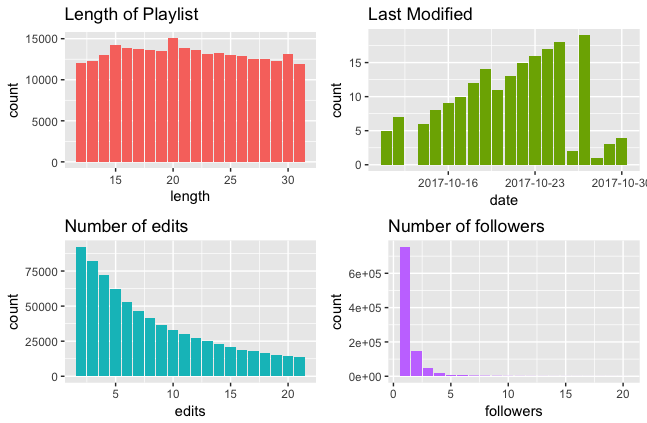
\includegraphics[width = 0.8\textwidth]{histograms.png}
  \caption{Histograms for selection of variables}
  \label{fig:boat1}
\end{figure}

%\subsection{Data Processing}

\section{Baseline}
\label{baseline}
My baseline model is a sequence-to-sequence model built from scratch following Tensorflow's Neural Machine Translation (seq2seq) Tutorial~\cite{luong17}.
This first version is a ``vanilla'' NMT model, with basic unidirectional single-layer LSTM recurrent network cells with $20$ units for both the encoder and the decoder. 
Below we show a diagram of our architecture, based on the neural machine translation architecture proposed by Luong~\cite{lmthang}.
\begin{figure}[ht]
	\caption{Network Architecture}
	\begin{minipage}[b]{0.55\linewidth}
		\centering
		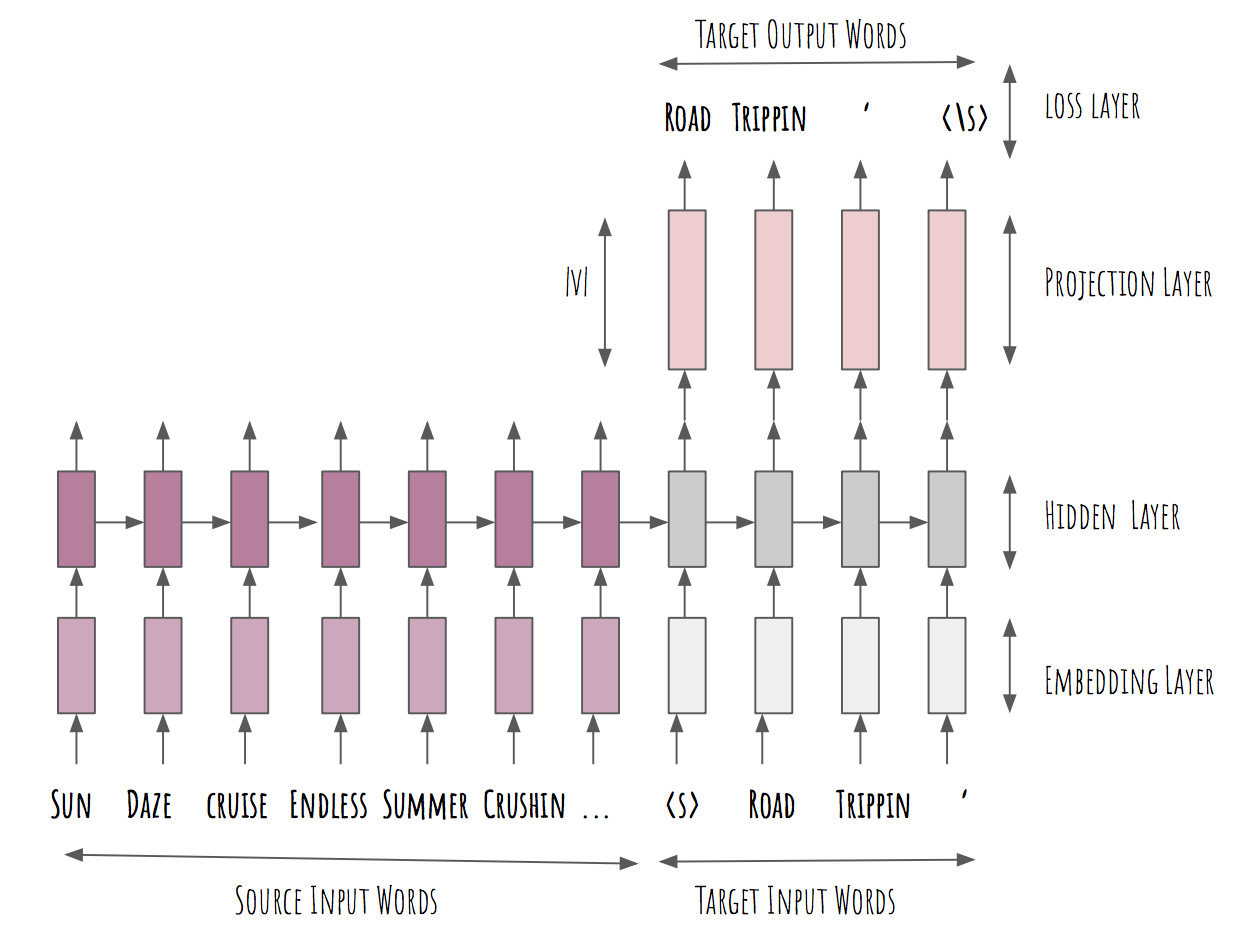
\includegraphics[width=\textwidth]{train-arch.png}
		\caption{Train Time}
		\label{fig:figure1}
	\end{minipage}
	\hspace{0.5cm}
	\begin{minipage}[b]{0.45\linewidth}
		\centering
		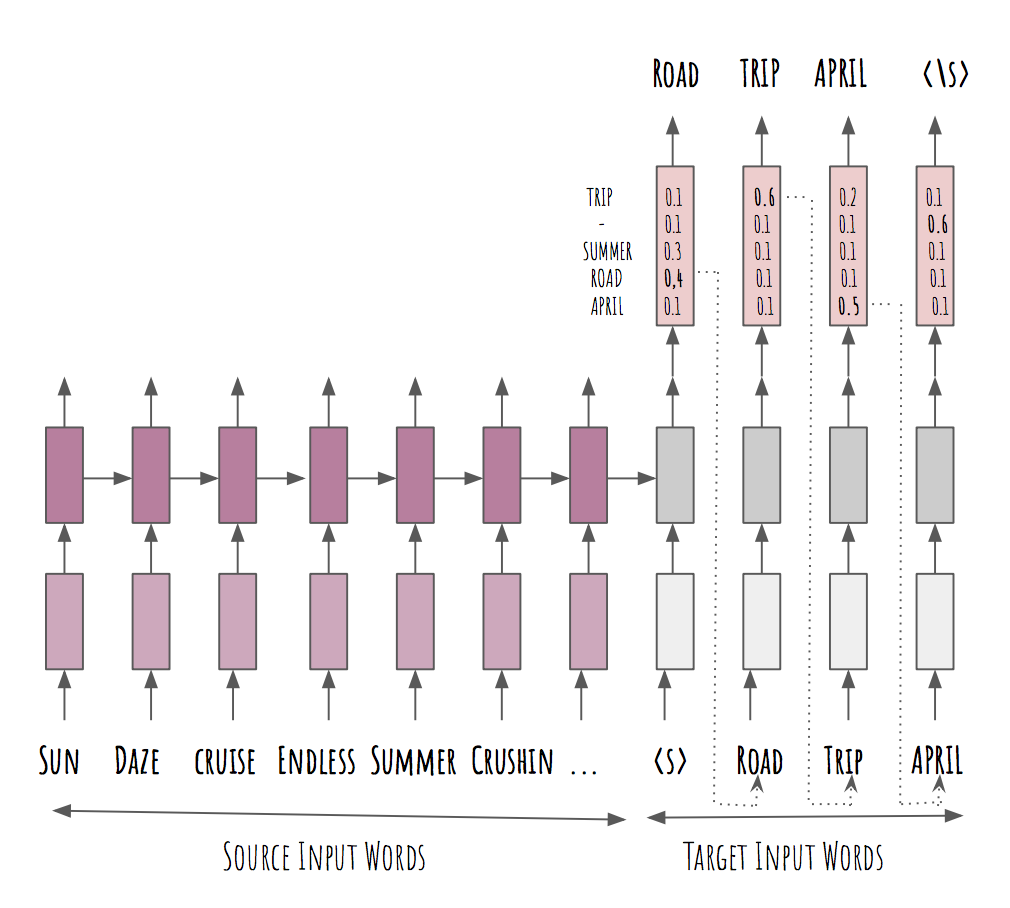
\includegraphics[width=\textwidth]{infer-arch.png}
		\caption{Inference Time}
		\label{fig:figure2}
	\end{minipage}
\end{figure}

Here, {\textless s \textgreater} marks the start of the decoding process while {\textless $\backslash$s\textgreater} tells the decoder to stop.
\begin{enumerate}[label = (\alph*)]
    \item \textbf{Embeddings}
        We initialize the embedding weights using pretrained GloVe vectors, which consist of a vocaulary of size $400,000$. 
		The embeddings are $100$-dimensional.
        We add four additional rows to the embedding matrix, corresponding to the following special tokens: 
        \begin{itemize}
            \item {\textless unk\textgreater}: Word representation for all words that appear in the track names and playlist titles but do not appear in our vocabulary.
            \item {\textless s\textgreater}: Word representation for the start token
            \item {\textless $\backslash$ s\textgreater}: Word representation for the end of sentence token 
            \item {\textless mask\textgreater}: Word representation for the mask or padding token.
        \end{itemize}
        These four rows are initialized to zero and the embeddings from these tokens are learned from scratch during training.
        As a next step, we consider to restricting the GloVe vocabulary to a smaller vocabulary size $V$ and only treating the most frequent $V$ letters as unique, while converting every other word to the {\textless unk\textgreater} token.
    \item \textbf{Encoder}
        The encoder takes the track names as inputs and does not make any predictions
        Specifically, the encoder receives as input the embedded source words; that is, the word representations of the padded concatenation of all the words in each tracklist of a playlist.
        The input tracklists are padded to a maximum length of $250$ words.
    \item \textbf{Decoder}
        The decoder processes the (target) playlist names while predicting the next words.
        It has access to the tracklist names through the final hidden state of the encoder.
        Additionally, during training, the decoder receives as input the playlist names padded to a maximum length of $10$ and shifted to the right by one word with an additional {\textless s\textgreater} token appended on the right. 
        During inference, we only have access to the tracklist (source), so we cannot feed the correct (shifted) playlist names as input to the decoder. 
        Instead, we use greddy decoding and feed the words predicted by the model in the previous timestep as input.
        We still use the last hidden step of the encoder to initialize the decoder, then feed a starting symbol token to the network to indicate the start of the decoding process and, in subsequent steps, feed the word with the maximum logit value out of the outputs of the decoder as input to the next timestep.
        The process continues until the end-of-sentence marker is produced or when we reach the maximum number of iterations. 
\end{enumerate}

The next steps would be to incorporate multi-layer LSTMs, add dropout, and use attention. 


\section{Evaluation Methodology}
\label{eval}

We will use as metric the $2$-gram overlap between automatically generated playlist titles and previous titles devised by humans, as proposed in NIST's annual Document Understanding Conferences (this metric is known as ROUGE: Recall-Oriented Understudy for Gisting Evaluation).
However, this could lead to bad scores for creative titles that no humans have come up with before.

\section{Results}
\label{results}
My model is currently running for $40$ epochs on the full dataset on the Azure GPU. I expect it to finish by Thursday.

\bibliographystyle{plain}
\bibliography{references}

\end{document}
